\textbf{COLUNI 2026 -- Questão 37}\par\medskip Analise os documentos abaixo:

\begin{center}Documento I\end{center}
\begin{minipage}{0.42\linewidth}
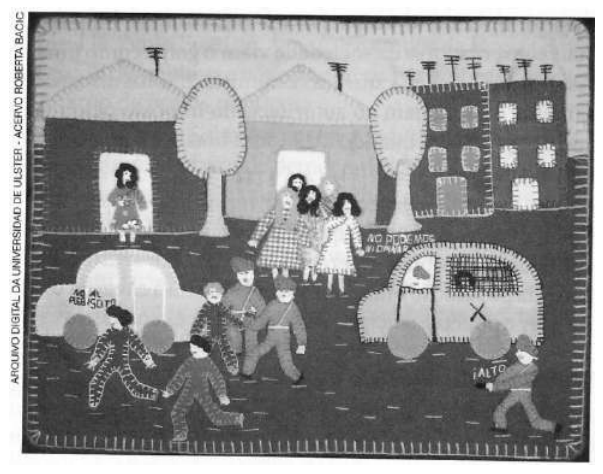
\includegraphics[width=\linewidth]{static/simulados/coluni/figuras/2026/questao-37/figura-1.png}
\end{minipage}\hfill
\begin{minipage}{0.54\linewidth}
“A arpillera é uma técnica têxtil (feminina) típica do Chile feita com tecidos rústicos, provenientes de sacos de farinha ou batatas, e costuradas a mão.”\par
APOLINÁRIO, Maria Raquel (org.). Projeto Araribá: história. São Paulo: Moderna, 9º ano, 2020, p. 225 (adaptado).\par
Ao lado, foto de uma arpillera chilena da década de 1970, na qual se vê policiais, homens e mulheres e as frases “Não podemos nem opinar”, “Não ao plebiscito”, “Alto”.
\end{minipage}

\begin{center}Documento II\end{center}
\begin{minipage}{0.32\linewidth}
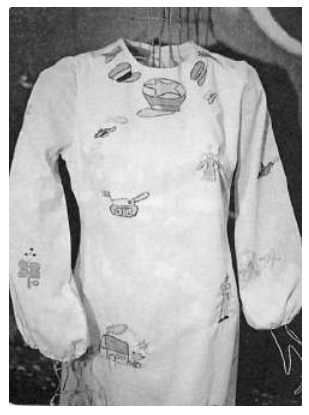
\includegraphics[width=\linewidth]{static/simulados/coluni/figuras/2026/questao-37/figura-2.png}
\end{minipage}\hfill
\begin{minipage}{0.63\linewidth}
“Zuleika Angel Jones (1921-1976), mais conhecida como Zuzu Angel, foi uma estilista brasileira [...]. Ela criou roupas inspiradas, principalmente, na cultura brasileira. Em uma de suas coleções, Zuzu Angel criou um vestido com estampas de desenhos infantis que mostravam pássaros na gaiola, anjos, crucifixos e tanques de guerra. Segundo ela, as roupas foram feitas em homenagem ao filho, Stuart Angel, assassinado.”\par
BRAICK, Patrícia Ramos. Estudar história: das origens do homem à era digital. São Paulo: Moderna, 9º ano, 2011, p. 246. (adaptado).\par
Ao lado, vestido da coleção Anjo Desamparado, Zuzu Angel, 1971.
\end{minipage}

Com base nos documentos acima e nos conhecimentos históricos, é INCORRETO afirmar que:\begin{enumerate}
\item as técnicas têxteis, como as \textit{arpilleras}, os bordados e a alta costura, por serem historicamente atividades sociais atribuídas ao gênero feminino, ficaram restritas ao ambiente doméstico, sendo utilizadas para a confecção de roupas e enxovais.
\item a \textit{arpillera} do documento I, e o vestido do documento II, foram artefatos produzidos por mulheres para denunciarem e protestarem contra a violência dos regimes militares da década de 1970 no Chile e no Brasil, respectivamente.
\item as mulheres foram protagonistas importantes em movimentos de contestação e resistência em países da América Latina, como Argentina e Chile que, assim como o Brasil, viveram períodos marcados por regimes militares.
\item a \textit{arpillera} e o vestido criado por Zuzu Angel foram instrumentos de manifestação política durante os regimes militares chileno e brasileiro, por utilizarem, em sua produção, detalhes que relacionavam o cotidiano à repressão, ao medo e à violência.\end{enumerate}